%!TEX root = ./main.tex
\section{Overview}
\label{sec2}

In this section, we firstly show an example of traditional resugaring approach. Then we will describe the framework of our whole approach, with two different approaches which work together and their separate examples.
\subsection{Existing resugaring method}
This subsection is original from \cite{resugaring} and \cite{hygienic}. But their original idea is from the first one, and the second one is a optimized version on hygienic macros and rewriting system.
\begin{Def}[Resugaring]
Given core language (named {\bfseries CoreLang}) and its evaluator, together with surface language based on syntactic sugars of CoreLang (named {\bfseries Surflang}). For any syntactic sugar, getting the evaluation sequences of the expression in SurfLang's syntax.It's not strict, so they use three properties for defining correctness.
\end{Def}
For correctness of the resugaring, the evaluation sequences should maintain the following three properties:
\begin{enumerate}
\item \emph{Emulation} Every surface term desugars to (a termisomorphic to) the core term it purports to represent.
\item \emph{Abstraction} If a term is shown in the reconstructedsurface evaluation sequence, then each non-atomic part of it orig-inated from the original program and has honest tags.
\item \emph{Coverage}  A sugar with good coverage shows many steps in the reconstructed surface evaluation sequence.
\end{enumerate}
It is a good summary for resugaring's properties, so we also use similar properties in our approach (using our domain).

Given an example to show how existing approach works. For syntactic sugar {\bfseries and} and {\bfseries or}, the sugar rules are:
\[
\begin{array}{l}
\drule{(\m{And}~e_1~e_2)}{(\m{if}~e_1~e_2~\false)}\\
\drule{(\m{Or}~e_1~e_2)}{(\m{if}~e_1~\true~e_2)}
\end{array}
\]
which forms a simple SurfLang.

The evaluation rules of {\bfseries if} is:
\[
\begin{array}{l}
(\m{if}~\true~e_1~e_2) \DeStep{e_1}\\
(\m{if}~\true~e_1~e_2) \DeStep{e_2}
\end{array}
\]
Then for SurfLang's expression $(\mbox{and}~(\mbox{or}~\#f~\#t)~(\mbox{and}~\#t~\#f))$ should get resugaring sequences as follow.

\begin{Codes}
    (and (or \#f \#t) (and \#t \#f))
\OneStep (and \#t (and \#t \#f))
\OneStep (and \#t \#f)
\OneStep \#f
\end{Codes}

The reason we should get the sequences above is because \Code{(and~(or~\#f~\#t)~(and~\#t~\#f))} should desugar to \Code{(if~(if~\#f~\#t~\#f)~(\mbox{if}~\#t~\#f~\#f)~\#f)}. Then in the CoreLang, the evaluation sequences will be as follow.
\begin{Codes}
    (if (if \#f \#t \#f) (if \#t \#f \#f) \#f)
\OneStep (if \#t (if \#t \#f \#f) \#f)
\OneStep (if \#t \#f \#f)
\OneStep \#f
\end{Codes}

The second item in the sequences can be desugared from $(\mbox{and}~\#t~(\mbox{and}~\#t~\#f))$, so resugars to it. So as the third item. In summary, the traditional approach firstly desugars the whole expression, then trys to transform the core sequences into surface sequences by match and substitution.

%Use a simple but sharp example to give an overview of your approach.
\subsection{Mixture Approach Framework}
We limit the language to s-expressions. Given an expression $\mbox{Exp} = (\mbox{Headid}~\mbox{Exp}*)$, the process of mixture approach will as Fig \ref{fig:mixture}.

\begin{figure}[t]
	\centering
	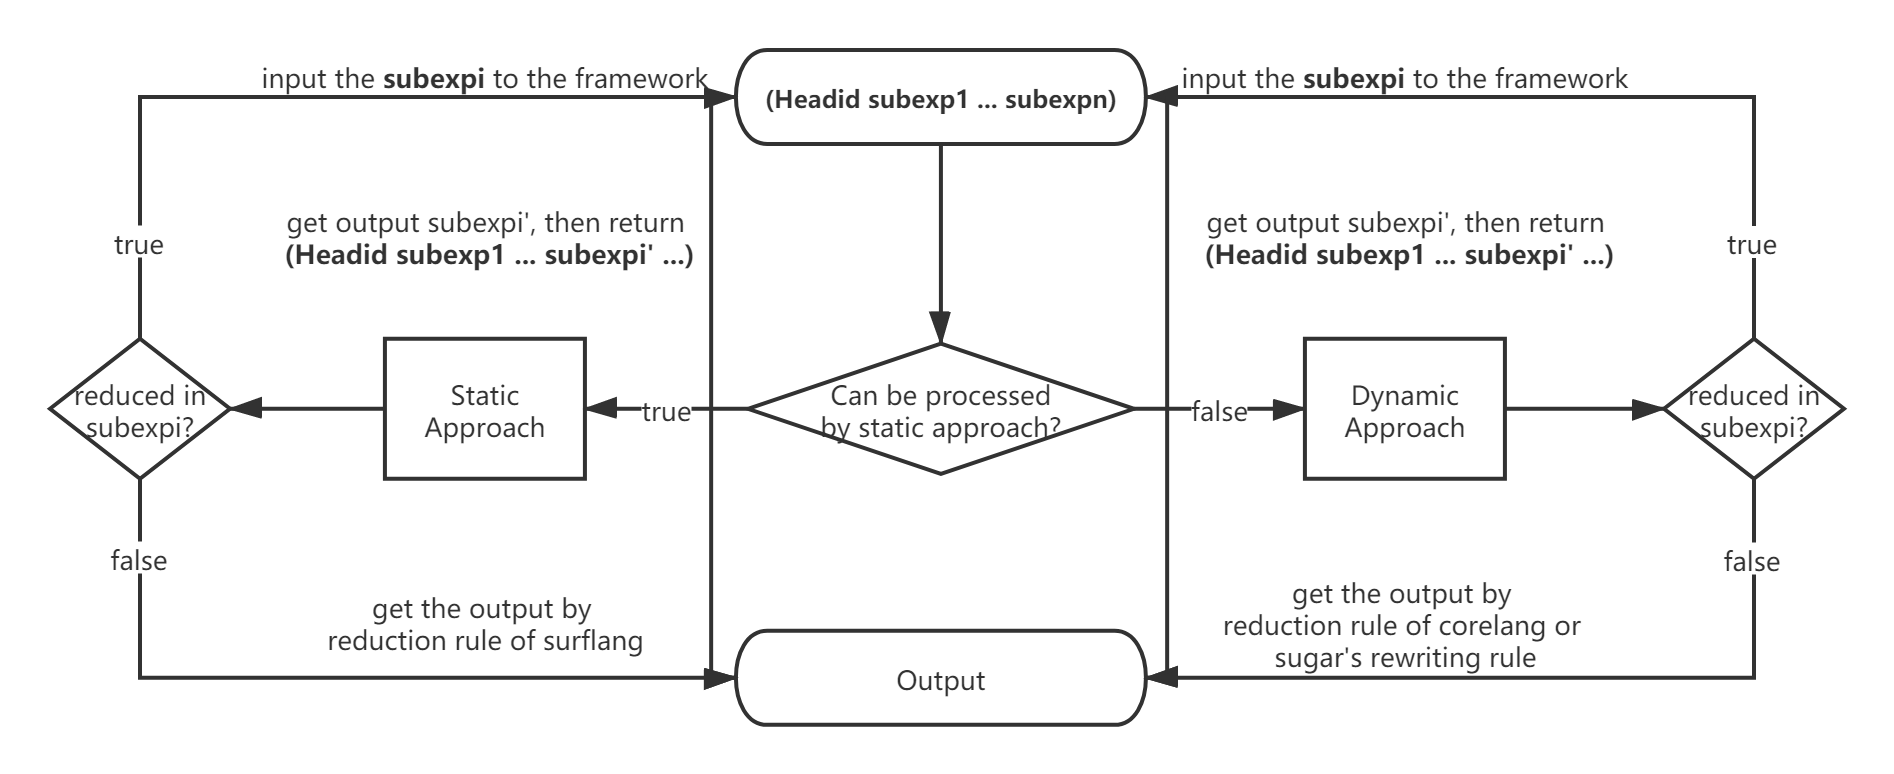
\includegraphics[width=12cm]{images/mixture.png}
	\caption{One step in framework of mixture approach}
	\label{fig:mixture}
\end{figure}

Given an example based on the former section. Besides sugar {\bfseries and}, {\bfseries or}, we add a recursive sugar {\bfseries mapf} based on another new sugar {\bfseries f}. The recursive sugar can be handled by the dynamic approach, but not for the static one. (Reasons in later sections)
\begin{Codes}
\small{(f e1 e2)} \DeStep{ (let x e1 (or x (and e2 x)))}
\small{(mapf e lst)} \DeStep{ (if (empty? lst) empty (cons (f e (first lst)) (mapf e (rest lst))))}
\end{Codes}

In the mapf (map of f) sugar, we use both core language's term (such as {\bfseries if, empty?, cons, let, first, rest}) and existing syntactic sugar ({\bfseries and, or}). The semantics of core language is as common. But to show some exact steps, we set the term {\bfseries cons} as a common expression (belonging to core language, but being displayed as surface language).


If we execute
\begin{Codes}
(mapf \#t (list \#f \#t))
\end{Codes}
 the mixture approach will judge whether sugar mapf can be handle by the static approach. No, then we use the dynamic approach in one step and get the intermidiate expression.
\begin{Codes}
    (mapf \#t (list \#f \#t))
\OneStep{ (cons (f \#t (first (list \#f \#t))) (mapf \#t (rest (list \#f \#t))))}
\end{Codes}
Then according to semantics of {\bfseries cons}, the first subexpression should be reduced. The subexpression can be handled by the static approach, so getting a subsequence.
\begin{Codes}
    (cons (f \#t (first (list \#f \#t))) (mapf \#t (rest (list \#f \#t))))
\OneStep{ (cons (f \#t \#f) (mapf \#t (rest (list \#f \#t))))}
\OneStep{ (cons \#t (mapf \#t (rest (list \#f \#t))))}
\end{Codes}
Then the second subexpression should be reduced, which is a recursive process. Finally, the subexpression (mapf \#t (list)) will be processed by dynamic approach.
\begin{Codes}
   (mapf \#t (list))
\DeStep{ (if (empty? (list)) empty ...)}
\OneStep{ empty}
\end{Codes}
Note that there are some steps should not be displayed, we define the common expressions above in syntaxs to restrict which intermediate step should be displayed.


The key idea of our dynamic approach, is that, regarding surface language and core language as a whole under the strategy of lazy desugaring. We design a core algorithm to choose the right reduction rule for any expression during the execution. Take the example
\Code{(and (or \#f \#t) (and \#t \#f))} again. We will get the sequence as Fig\ref{fig:core-algo}.

\begin{figure}[ht]
\parbox[t]{\textwidth}{
\begin{Codes}
    (and (or \#f \#t) (and \#t \#f)) $\dashrightarrow_{step1}$
(and (if \#f \#t \#t) (and \#t \#f)) $\dashrightarrow_{step2}$\\
(and \#t (and \#t \#f)) $\dashrightarrow_{step3}$
(if \#t (and \#t \#f) \#f) $\dashrightarrow_{step4}$
(and \#t \#f) $\dashrightarrow_{step5}$\\
(if \#t \#f \#f) $\dashrightarrow_{step6}$
\#f
\end{Codes}
		}
\caption{core-algo example}
\label{fig:core-algo}
\end{figure}

At step 1, we found the outermost $and$ sugar don't have to expand, because its first sub-expression will reduce earlier. At step 2, the same as step 1. At step 3, the outermost $and$ sugar have to expand, because no sub-expression will reduce after the whole expression desugar. At step 4, the inner $and$ sugar don't have to expand either. At step 5, the sugar have to desugar to CoreLang. Finally at step 6, we get the final result. Note that there are some sequences which should not be shown, we use another function to filter them.

The key idea of our static approach, is that, converting reduction semantics of core language into automata (called \emph{IFA}), building IFA for syntactic sugar, converting the IFA of sugars into reduction semantics. It is an abstract of dynamic approach in a sence, we will discuss it in Sec\ref{sec6}. Take another {\bfseries or} sugar for example.

\[
\begin{array}{l}
\drule{(\m{or}~e_1~e_2)}{(\m{let}~x~e_1~(\m{if}~x~x~e_2))}
\end{array}
\]
where the rules of \emph{if} and \emph{let} is the same following

\[
\begin{array}{l}
\drule{(\m{if}~\true~e_1~e_2)}{e_1}\\
\drule{(\m{if}~\true~e_1~e_2)}{e_2}
\end{array}
\]
\ignore{
The {\bfseries let} and {\bfseries if} expressions' reduction semantics can be represented as  the following automata.

\begin{tikzpicture}[->,>=stealth',shorten >=1pt,auto,node distance=2.8cm,
semithick]
\tikzstyle{every state}=[circle,draw,minimum size=16pt,font=\large]

\node[initial,state] (A) {$e_{1}$};
\node[state,accepting] (B) [above right of=A] {$e_{2}$};
\node[state,accepting] (C) [below right of=A] {$e_{3}$};

\path (A) edge node {\#t} (B)
edge node {\#f} (C)
edge [loop above] node {} (A)
;

\end{tikzpicture}


\begin{tikzpicture}[->,>=stealth',shorten >=1pt,auto,node distance=2.8cm,
semithick]
\tikzstyle{every state}=[circle,draw,minimum size=16pt,font=\large]
\node[initial,state] (A) {$e_{1}$};
\node[state,accepting](B)[right of=A,align=center, font=\small ]{$e\_2_{v}^{x}$}[above];
%\node at (-0.5,1)[draw, align=center]{example \\ example example};

\path[]
(A) edge node {$v$} (B)
(A) edge [loop above] node {} (2);

\end{tikzpicture}

Then for {\bfseries Or} sugar, we merge the IFA of if expression into node {$e_2$} of let's IFA.

\begin{tikzpicture}[->,>=stealth',shorten >=1pt,auto,node distance=2.8cm,
semithick]
\tikzstyle{every state}=[circle,draw,minimum size=16pt,font=\large]

\node[initial,state] (A) {$e_{1}$};
\node[state] (D) [right of=A,font=\small] {$x_{v}^{x}$};
\node[state,accepting] (B) [above right of=D,font=\small] {$x_{\#t}^{x}$};
\node[state,accepting] (C) [below right of=D] {$e_2$};

\path[]
(A) edge node {$v$} (D)
(A) edge [loop above] node {} (A)
(D) edge node {$\#t$} (B)
(D) edge node {$\#f$} (C);

\end{tikzpicture}
}
From the IFA of or expression, we can get the following reduction semantics.
\[
\begin{array}{l}
\infer {(\mbox{Or}~e_1~e_2) \rightarrow (\mbox{Or}~e_1'~e_2)} {e_1~ \rightarrow~e_1'}\\
(\mbox{Or}~\#t~e2) \rightarrow \#t \\
(\mbox{Or}~\#f~e2) \rightarrow e_2 \\
\end{array}
\]

Then the resugaring sequences can be get by the reduction semantics.
